\documentclass[%
 reprint,
 amsmath,amssymb,
 aps,
]{revtex4-2}

\usepackage{graphicx}% Include figure files
\usepackage{dcolumn}% Align table columns on decimal point
\usepackage{bm}% bold math
\usepackage{hyperref}% add hypertext capabilities
\usepackage{graphicx}
\usepackage{color}

%\preprint{APS/123-QED}
\begin{document}
\title{Acoustics I project: rotating and resonant waves in a cylindrical cavity}
\author{Mathieu Maréchal\\ Supervisor: Guillaume Penelet}
\affiliation{
    M1 Wave Physics \& Acoustics\\Le Mans Université
}%
\date{\today}

\begin{abstract}
    \textbf{Abstract:} In this paper, we study a cylindrical cavity in which we derive analytical solutions using the modal expansion method for the emission of acoustic waves by a loudspeaker. Using these solutions, we can generate a field from several sources and investigate the layouts for the speakers that leads to a rotating mode. A general layout was found to create a rotating mode for any number of loudspeaker in the cylinder. Finally, an extension of the model to 3D was proposed.
\end{abstract}

\maketitle
\section{Introduction}
Cylindrical waveguides and modal analysis were among the key notions tackled in the Acoustics I class. And what better way to make use of these two notions than to study rotating waves. This present paper describes the project led within the framework of this course, dealing with resonant and rotating waves in a cylindrical resonant cavity. Rotating waves are not a very hot topoc within the acoustics research topics, they are more dealt with for quantum and electromagnetic waves. However, they were studied by Ceperley \cite{ceperley2002} who introduces rotating waves for water and for acoustics. The same phenomenon can also be generated and observed for other types of waves: an electromagnetic resonator can also have rotating modes \cite{ceperley1995}. One interesting aspect to this type of wave is that it transfers its angular momentum to matter as studied by \emph{Santillan et al.} \cite{santillan2009}. What follows will focus on the ways to generate an acoustic vortex or in other words, a rotating wave field. This study will be done in several parts. Firstly, one has to study analytically the characteristics of the considered cylindrical cavity, and in particular its nodal lines for specific modes, along which the point sources generating the rotating field will be placed. Then, making use of the superposition principle, one will be able to numerically simulate several phase-shifted sources exciting the cavity. Finally, controlling the phasing of these sources, one should be able to control the nature of the wave propagating in the cavity, thus allowing the production of a vortical wave field. 

\begin{figure}
    \centering
    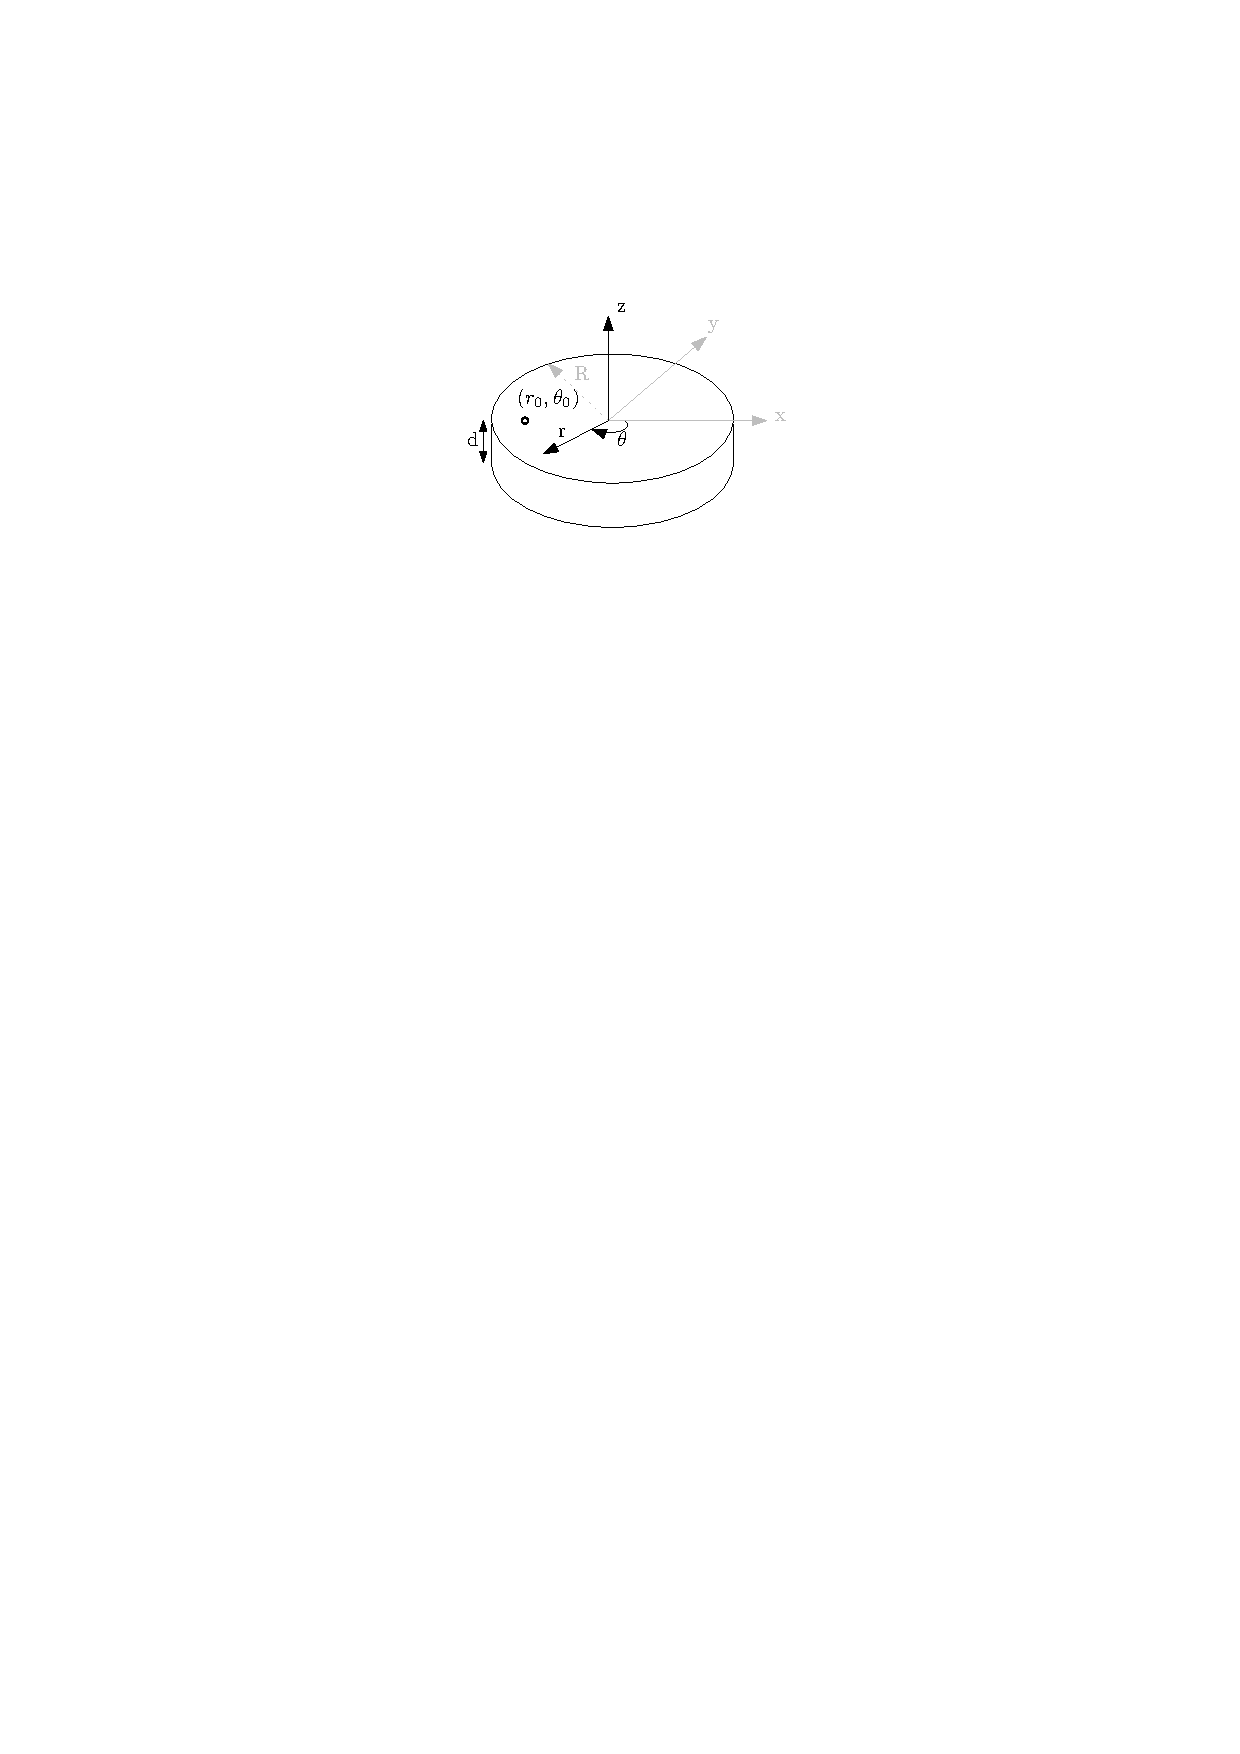
\includegraphics[width=.35\textwidth]{figures/schema.pdf}
    \caption{Representation of the cylindrical cavity of radius $R$ and height $d$ with one point source at $(r_0, \theta_0)$}
    \label{fig:schema}
\end{figure}

\section{Derivation of the pressure field inside the cylinder using modal analysis}
The system considered in this paper is a cylinder which includes one (and thereafter several) loudspeaker seen as a point source located at $\vec{r}_0 = (r_0, \theta_0, z_0)$ creating an acoustic field $\tilde{p}(\vec{r}, t)$, $\vec{r} = (r, \theta, z)$. This point source imposes a driving force $q_0$ oscillating at a $\omega$ frequency. The cylinder is filled with air, a lossless medium with density $\rho_0 = 1.2$ kg.m$^{-3}$ and sound celerity $c_0 = 343$ m/s. Its radius is denoted $R$ and its length as $d$. A representation of the studied system is proposed in figure \ref{fig:schema}.

\subsection{Modal expansion in the two-dimensional case}
During this part, a 2D pressure field $\tilde{p}(r, \theta)$ will be considered: it will only depend on its azimuthal $\theta$ and radial $r$ coordinates, and we will write that $d \ll R$. The wave equation to solve in the cavity is inhomogenenous,
\begin{equation}
    \begin{split}
        \frac{\partial \tilde{p}^2}{\partial r^2} + \frac{1}{r} \frac{\partial \tilde{p}}{\partial r} &+ \frac{1}{r^2} \frac{\partial \tilde{p}^2}{\partial \theta^2} + k^2 \tilde{p}\\ &= -i \omega q_0 \delta(r - r_0) \delta(\theta - \theta_0),
    \end{split} \label{eq:2dwaveq}
\end{equation}
with $k = \omega/c_0$ the wavenumber and $\delta$ is the Dirac-Delta distribution.
The edges of the cavity are all considered rigid, thus giving the following boundary conditions on the acoustic field
\begin{equation}
   \begin{split}
       \tilde{p}(r, \theta + 2 \pi) &= \tilde{p}(r, \theta),\\
               \left. \tilde{v}_r \right|_{r=R} & = 0 \Rightarrow J'_m (k_{mn}R) = 0.
   \end{split} \label{eq:bc2d}
\end{equation}
Due to the periodicity condition, we have that the clockwise and anticlockwise spinning modes $m \in \mathbb{Z}$ are integers. Furthermore, due to the Bessel functions properties stating that $J_m = (-1)^m J_{-m}$ the same order symmetric modes $m$ and $-m$ are eigenpairs and share the same eigenvalues \cite{rona2007}, so that $m \in \mathbb{N}$.

The solution of the field can be written by making use of the modal analysis method, which tells that any pressure field can be generally written as 
\begin{equation}
    \tilde{p}(r, \theta) = \sum_{m,n} \tilde{C}_{mn} \Psi_{mn}.
\end{equation}
Where $\tilde{C}_{mn}$ is a term representing the amplitude of the field, and $\Psi_{mn}$ are the eigenfunctions, determined using the boundary conditions from equation (\ref{eq:bc2d}). Using $\Psi_{mn} = \tilde{C}_{mn} J_m (k_{mn}r)\left[ \tilde{A}_{\theta m} \cos(m \theta) + \tilde{B}_{\theta m} \sin(m \theta) \right]$ as the set of eigenfunctions, we will be able to find the expression of the amplitude terms. To do that, one has to orthogonalize or normalize each part of the eigenfunction.

To begin with, in order to make calculations a bit simpler, the eigenfunction can be rewritten as
\begin{equation}
        \tilde{p}(r, \theta) = \sum_{mn}^{\infty} J_m(k_{mn}r) \left[ \tilde{A}_{mn} \cos(m \theta) + \tilde{B}_{mn} \sin(m \theta) \right], \label{eq:gensol}
\end{equation}
where the amplitude term $\tilde{C}_{mn}$ can be expressed inside $\tilde{A}_{\theta_{mn}}$ and $\tilde{B}_{\theta_{mn}}$, which were thus respectively renamed $\tilde{A}_{mn}$ and $\tilde{B}_{mn}$.

Subsequently, the pressure field written in equation (\ref{eq:gensol}) can be put in equation (\ref{eq:2dwaveq}), which leads to
\begin{equation}
    \begin{split}
        \sum_{mn} &\left[ k^2 - k_{mn}^2 \right] J_m(k_{mn}r) \Big[ \tilde{A}_{mn} \cos(m\theta) \\&+ \tilde{B}_{mn} \sin(m\theta) \Big]= - i \omega_0 q_0 \delta(r - r_0) \delta(\theta - \theta_0)
    \end{split} \label{eq:rawsol}
\end{equation}

Now to the orthogonalization part: we will here proceed to normalize each part of the eigenfunction using the following scalar product results 
\begin{equation}
   \int_0^{2 \pi} \cos^2\left( m \theta \right) d\theta = 
    \begin{cases}    
        2 \pi, & m = 0\\
        \pi, & m \ne 0
    \end{cases}, \label{eq:dp_2}
\end{equation}

\begin{equation}
    \int_0^{2 \pi} \sin^2\left( m \theta \right) d\theta = 
    \begin{cases}    
        0, & m = 0\\
        \pi, & m \ne 0
    \end{cases}, \label{eq:dp_3}
\end{equation}
and one property of the Bessel function is\cite{abramsteg}
\begin{equation}
    \begin{split}
        \int_0^{R} &r J^2_m (k_{mn} r)dr \\ &=
    \begin{cases}    
        \quad  \quad \quad 1/2, & k_{mn}R = 0\\
        \frac{k^2_{mn} R^2 - m^2}{2 k^2_{mn}} J^2_m (k_{mn} R), & k_{mn}R \ne 0
    \end{cases}.
    \end{split} \label{eq:dp_4}
\end{equation}

These results can be used in our calculations. Therefore, they are rewritten in a more aesthetic and usable way using the Kronecker delta symbol defined as 
\begin{equation}
   \delta_i^j = \begin{cases}
       1, & i = j\\ 0, & i \ne j
   \end{cases}.
\end{equation}

With this notation, equations (\ref{eq:dp_2}) and (\ref{eq:dp_3}) are respectively equal to $\pi(1 + \delta_m^0)$ and $\pi(1 - \delta_m^0)$. Finally, the case for $k_{mn}R = 0$ in equation (\ref{eq:dp_4}) can be discarded as it is a solution that is trivial (nothing is happening in the cavity).

These operations can be also simply described as an integration over the surface of the studied disk and a multiplication of the equation (\ref{eq:rawsol}) with successively $r J_m(k_{mn}r) \cos(m\theta)$ in order to retrieve $\tilde{A}_{mn}$ and $r J_m(k_{mn}r) \sin(m\theta)$ to get $\tilde{B}_{mn}$. After the application of these operations, we end up with
\begin{equation}
    \begin{split}
        \tilde{A}_{mn} =& \frac{- 2 i \omega_0 q_0 r_0}{\pi (1 + \delta_m^0)} k_{mn}^2  \cos(m \theta_0) \frac{J_m(k_{mn}r_0)}{J^2_m(k_{mn}R)}\\ &\times\left[(k^2 - k^2_{mn}) ((k_{mn}R)^2 - m^2)\right]^{-1}
    \end{split}
\end{equation}
and 
\begin{equation}
    \begin{split}
        \tilde{B}_{mn} =& \frac{- 2 i \omega_0 q_0 r_0}{\pi (1 - \delta_m^0)} k_{mn}^2  \sin(m \theta_0) \frac{J_m(k_{mn}r_0)}{J^2_m(k_{mn}R)}\\ &\times\left[(k^2 - k^2_{mn}) ((k_{mn}R)^2 - m^2)\right]^{-1}
    \end{split}
\end{equation}

The expression for the two amplitude terms can be used in equation \ref{eq:gensol} and the pressure field of a point source can be calculated. This will be implemented in a Python script which will allow us to visualise the mode shapes of the cylindrical cavity. %and will be the basis for any extension of this simulation.  

\section{Resonant modes of the cavity and influence of the point source}
\subsection{Investigation with one source: mode shapes}
Now that the pressure field expression was derived, one can make use of this analytical solution to plot the resonance modes of the cylindrical cavity. A figure can be constituted for a range of modes $mn$ from 10 to 22, and is presented in figure \ref{fig:modes}. For modes $n>1$, there is one or more nodal circle in the cylinder as well as some nodal lines. The higher the mode $mn$ is, the more localized the pressure maximas and minimas will be. The shape of the modes on figure \ref{fig:modes} are quite close to the fundamental patterns given by $J_m(k_{mn})\cos(m\theta)$ (as represented in the lecture notes). The difference with the original modal shapes are that the cavity is here excited by a point source: the excitation frequency and the geometry is changed. Indeed, the excitation frequency of the source cannot be strictly the same as a given mode resonance frequency due to the term $\left.\left[k^2 - k^2_{mn}\right]^{-1}\right|_{k = k_{mn}} \longrightarrow \infty$ in the amplitudes equations. Indeed, this doesn't do good with computer simulations, so we restrain ourselves with a close-enough value for $k \approx k_{mn}$ in order to mostly excite the mode we want to observe.

Also, the position of the source has an influence on the pressure distribution along the disk: the nodes closer to the source have a higher amplitude than the one that are away, it's not perfectly symmetric. 

\begin{figure}
    \centering
    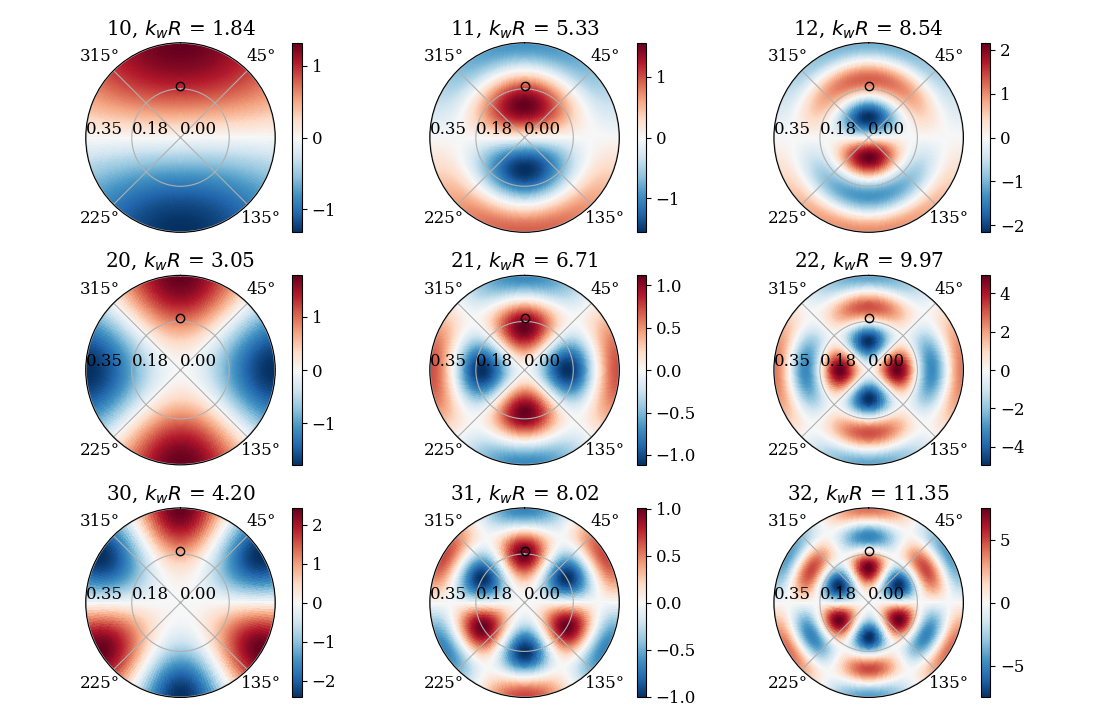
\includegraphics[width=.5\textwidth]{figures/modes.png}
    \caption{Modes $m,n$ of the cavity generated by a single point source represented by a black hollow circle. The source is located at ($r_0$ = $R/2$, $\theta_0$ = $\pi$) and emits a flow $q_0 = 10^{-2}$ m$^3$/s with a frequency close to the resonance of each mode $\omega_0 = c_0 \: (k_{mn} + 0.1)$. The real pressure field is normalized with respect to the pressure at the point source.}
    \label{fig:modes}
\end{figure}

\subsection{Investigation with one source: position in the cavity}
An important part of the simulations is the positioning of the source inside the cavity, which we need to understand if we want to generate rotating waves. We saw how the slight difference between the excitation frequency and the frequency of the resonator's mode influences the modal shape. The position has an impact too: in the previous figure where the point source was located at $(R/2, \pi)$, the mode shapes were quite consistent with pure mode shapes. However, positioning the source in different locations yields very different shapes.

In figure \ref{fig:source_pos}, the source was positioned at four noteworthy locations. The sources for \ref{fig:source_pos}a. and \ref{fig:source_pos}d. were placed at the center of a node where maximum pressure was noticed; for \ref{fig:source_pos}b. and \ref{fig:source_pos}c. the source was placed so that it was along a nodal line from what we could observe on the mode 21 shape on figure \ref{fig:modes}. For \ref{fig:source_pos}d., the source was at the intersection between a nodal line and a nodal circle and close to the center. As it turns out, the modal shape rotates with the source $\theta$ angle position: a node is always located at the source position with its shape rotated of the same angle. We can therefore conclude that no source can be located along one of the transversal nodal lines except if it's closer to the center, the nodal circle for mode 11, 21, \ldots is also changed with the source position.

The position of the node of the mode 21 does not seem to be influenced by the radial position of the source even if its shape gets larger as can be seen on figure \ref{fig:source_pos} where the source is along the second nodal circle and the 2 nodes are kind of fused together.

From these observations, the proper definition of the azimuthal coordinate of the source is an important parameter to promote the generation of rotating waves. The other one, which was not discussed up to now, is the phase of each of the point sources and it will be discussed in the next part.

\begin{figure}[h]
    \centering
    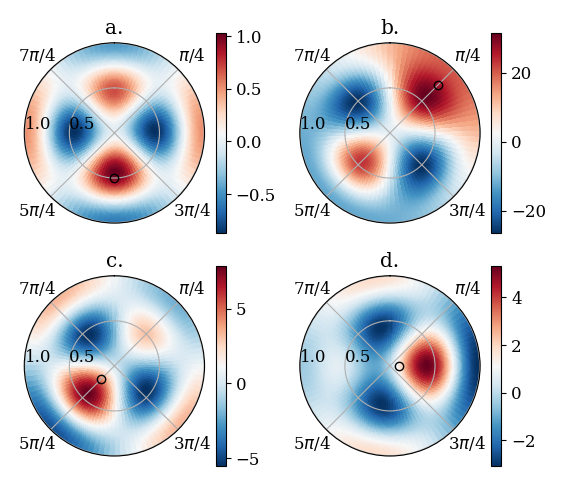
\includegraphics[width=.5\textwidth]{figures/source_pos.png}
    \caption{Pressure distribution for the mode 21 in the cavity for different source positions. The source in all cases emits a flow $q_0 = 10^{-2}$ m$^3$/s with a frequency $\omega_0 = c_0 \: (k_{mn} + 0.03)$. The position of the source for each subfigure is: a. $(0.5, \pi)$, b. $(0.75, \pi/4)$, c. $(0.2, 5 \pi/4)$, d. $(0.1, \pi/2)$. The normalisation of the amplitude was the same as the previous figure.}
    \label{fig:source_pos}
\end{figure}

\subsection{Adding more sources in the cavity}
In order to generate rotating waves, one has to put more than one loudspeaker in the cavity. Doing so from the previous simulations is fairly easy: one simply need to make use of the superposition principle as the studied system is linear. The additivity property states that the pressure field generated by several sources will be the sum of the pressure field generated by each source. One will set their behaviour to depend on the same parameters $q_0$ and $k$. Each source is governed by the same equations we studied beforehand and the field generated by each will interact with one another. What will be done in the next part is to study how to tune each source regarding the others to generate an acoustic vortex. The varying parameters for each source is its azimuthal location $\theta_0$ and its phase $\phi_0$. The phase is used to define the time-varying pressure field
\begin{equation}
    \tilde{p}(r, \theta, t) = \Re\left[\tilde{p}(r, \theta)\right] e^{i (\omega t - \phi_0)}
\end{equation}
where $\tilde{p}(r, \theta)$ is the pressure field defined at equation (\ref{eq:gensol}) and $\phi_0$ is the phase of the source.

\section{Simulating rotating waves in the cavity}
The observation of rotating waves is the core part of this project. The goal of this part is to investigate the way to promote their generation. In this part the $\theta_0$ location of a given source $i$ will be denoted $\theta_0^{(i)}$ and its phase $\phi_0$ is written $\phi_0^{(i)}$. From the two articles mentioned before, one can already make use of some configurations of the sources that were used to observe rotating modes. Ceperley states \cite{ceperley2002, ceperley1995} that 2 sources with a phase lag of $\pi/2$ and an angle of $\pi/2$ between them will create a purely rotating mode for any mode having a nodal circle. From \emph{Santillo et al.}, there are some configuration for rotating modes with 4 and 8 sources, which were tested in free field. Finally, in the outline is described a configuration which would use 3 sources with a phase of $\phi_0^{(2)} = 2\pi/3$ and $\phi_0^{(3)} = 4\pi/3$ with $\theta_0^{(2)} = 2\pi/3$ and $\theta_0^{(3)} = 4\pi/3$ with respect to the first source. These layouts will be used to confirm our approach.

In order to validate the newly developed model to generate rotating wave, one can use the geometry which uses 4 sources, which is described extensively in the paper. The simulation was processed using exactly the parameters for angles and phases noted for this configuration and uses the mode 10 of the cavity. The result is presented in figure \ref{fig:contour_time}. With the sources exciting the mode 10, waves rotates in the clockwise direction and the rotation of the mode has a period $T = 0.01$ s (the mode 10 corresponds to an excitation frequency $f_{10} = 992$ Hz).

A configuration with 2 sources when they have an angle $\theta = \pi$ (wherever along the disk) and a phase $\Delta \phi = \pi/2$ yields to a purely rotating mode, which was tested for several low order $m,n$ modes. What was observed is that gradually varying the phase of one of the sources allows for a combination of a standing and a rotating wave. The wave will gradually take the form of a standing mode until the phase is $\Delta \phi = \pi$ and it becomes a purely standing wave. One remark on the rotation of the waves is that it's not constant when they are combined to a standing wave; the rotation velocity is lower when the nodes and antinodes are at their maximum and it accelerates when the amplitude of the nodes and antinodes are closer to the amplitude of the nodal lines (in other words, when the pressure field becomes zero everywhere). On the whole, the rotation speed of the waves is directly linked to the excitation frequency: higher mode seems to lead to a faster rotation of the field.

\begin{figure}
   \centering 
   \def\svgwidth{0.45\textwidth}
   \input{contour_time.pdf_tex}
   \caption{Rotation of waves inside the cavity with 4 sources emitting an acoustic wave with each its own phasing. a) Representation of the pressure distribution of the mode 10 for 4 successive time values: 1.3 ms (shading of purple lines), 1.8 ms (shading of blue lines), 2.3 ms (green) and 2.8 ms (orange). The sources are represented in the graph with their respective phase. 2 squares (1) and (2) are measure points where the pressure evolution with time is displayed in b), normalized with the maximal pressure at (1).} 
   \label{fig:contour_time}
\end{figure}

\subsection{Generalisation of the arrangement to $n$ sources}
The previously proposed layouts for the source positions seems to show that there is a possible general pattern for the generation of vortical waves. Indeed, given a number of source $n \ge 2$, we can generte a purely rotating mode if
\begin{equation}
    \theta^{(i)} = \frac{2 \pi i}{n}, \quad \text{and} \quad \phi^{(i)} = \frac{2 \pi i}{n}.
    \label{eq:gener_n}
\end{equation}
where $i = 0 \ldots n-1$ is the index of the source and $n$ is the total number of sources to put inside the cavity. Here $\theta^{(i)} = \phi^{(i)}$ but it does not mean that there can not be a layout of sources with $\theta^{(i)} \ne \phi^{(i)}$ that wouldn't work.

Any arrangement having azimuthal positions and relative phases following the equation (\ref{eq:gener_n}) will produce a purely rotating mode inside the cavity. Indeed, the layouts with 2, 3 and 4 sources verify this equation. Testing with 25 sources leads also to a purely rotating mode. 4 frames with different time values of the animation of the 22 mode being excited with this number of sources are presented on figure \ref{fig:pleindesources}. 

\begin{figure}
    \centering
    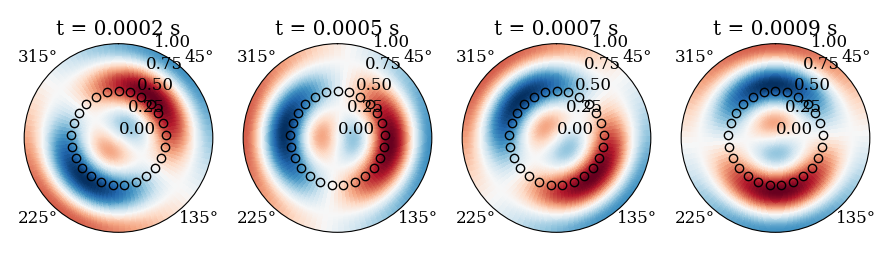
\includegraphics[width=0.5\textwidth]{figures/pleindesources.png}
    \caption{Example of the generation of a purely rotating mode using a layout of 25 sources. The pressure field ranges between $\pm 0.6$ Pa with loudspeakers having each a mass flow rate $q_0 = 0.001$ m$^3/$s. The first source $s_0$ has a position 0 and a zero phase and for instance the last source $s_{24}$, $\theta^{(24)} = \frac{48\pi}{25}$, $\phi^{(24)} = \frac{2 \pi i}{n}$}
    \label{fig:pleindesources}
\end{figure}

\section{Extension of the study to 3D}
In order to extend the previous equations to the three dimensional case, the first thing to do is that one has to add a boundary condition at $z=0$ and $z=d$: each end of the cylinder is considered rigid so that $\left. \tilde{v}_z \right|_{z=0} = \left. \tilde{v}_z \right|_{z=d} = 0$. The wavenumber becomes then  $k^2 = k_{mn}^2 + k_z^2$, with $k_z = \frac{l \pi}{d}$

The general equation for the pressure field is
\begin{equation}
    \begin{split}
        \tilde{p}(r, \theta, z) &= \sum_m^{\infty}\sum_n^{\infty}\sum_l^{\infty} J_m(k_{mn}r) \cos(k_z z)\\ &\times \left[ \tilde{A}_{mnl} \cos(m \theta) + \tilde{B}_{mnl} \sin(m \theta) \right],
    \end{split}
\end{equation}

and the source term of the wave equation in (\ref{eq:2dwaveq}) becomes $-i\omega q_0 \delta(\vec{r} - \vec{r_0})$, with $\vec{r} = (r, \theta, z)$ and $\vec{r}_0 = (r_0, \theta_0, z_0)$ is the vector of the position of a source $s_0$. Using the same approach to retrieve the amplitude expressions, one has to use the previous scalar products used in the derivation of the pressure field in the 2D case as well as a new one for the $\cos(k_z z)$ term, which is $\int_0^l \cos^2\left( \frac{l \pi}{d}z \right) dz = d/(2 - \delta_l^0)$ using the Kronecker-Delta notation already used for the 2D equations. The pressure field then has to be integrated over the volume of the cylinder and multiplied by $r J_m(k_{mn}r) \cos(m\theta) \cos(k_z z)$ to get $\tilde{A}_{mnl}$ and similarly with a $\sin(m\theta)$ term for $\tilde{B}_{mnl}$. Thus, the solution for the amplitude terms can be written as 
\begin{equation}
    \begin{split}
        \tilde{A}_{mnl} = &\frac{- i 2 q_0 \omega r_0 k^2_{mn} \cos(k_z z_0) \cos(m \theta_0)}{\pi d\left[k^2 - k^2_{mn} - k^2_z \right] \left[(k_{mn}R)^2 - m^2 \right]}\\  &\times \frac{2 - \delta_l^0}{1 + \delta_m^0} \frac{J_m(k_{mn}r_0)}{J^2_{m}(k_{mn}R)},
    \end{split}
\end{equation}
and
\begin{equation}
    \begin{split}
        \tilde{B}_{mnl} = &\frac{- i 2 q_0 \omega r_0 k^2_{mn} \cos(k_z z_0) \sin(m \theta_0)}{\pi d\left[k^2 - k^2_{mn} - k^2_z \right] \left[(k_{mn}R)^2 - m^2 \right]}\\  &\times \frac{2 - \delta_l^0}{1 - \delta_m^0} \frac{J_m(k_{mn}r_0)}{J^2_{m}(k_{mn}R)}.
    \end{split}
\end{equation}
Similar study can be done for the whole cylinder but it is very similar with the 2D case. However, such simulations reach the limitations of the Python graphical library \emph{Matplotlib} used for the other figures of the report, with which it's not possible to generate contour lines over a volume. This would require another library such as Plotly which seems to make this possible or Matlab.

\section{Conclusion}
Some perspectives and ideas that could be tapped to extend this project are first of all an experimental setup in order to actually observe this phenomenon in real life. A FEM simulation could be run also in order to validate the analytical results and would probably be a better way to simulate rotating modes in a three dimensional cavity as it is tedious to do so using analytical solutions with a programming language as Python or Matlab.

Some more fundamental aspects of the topic could be broadened: for example, what produces a combination of a rotating and a standing mode and how the phase of each source influences this behaviour. This could be done by further digging into the literature or by experiment with a more rigourous approach to determine which position and phase arrangement will give a rotating mode. 

The content of this project including the scripts as well as some animations are available on a Github repository: \url{https://github.com/marecmat/VorticalWavesAcoustics}.

\bibliography{biblio}


\end{document}
